\documentclass[conference]{IEEEtran}
\IEEEoverridecommandlockouts
\usepackage{cite}
\usepackage{amsmath,amssymb}
\usepackage{graphicx}
\usepackage{booktabs}
\usepackage{textcomp}
\usepackage{xcolor}
\usepackage{url}
\usepackage{balance}
\graphicspath{{figs/}}
\def\BibTeX{{\rm B\kern-.05em{\sc i\kern-.025em b}\kern-.08em T\kern-.1667em\lower.7ex\hbox{E}\kern-.125em X}}


\begin{document}

\title{Machine-Learning-Based Noise Source Fingerprinting for Quantum Circuits:\\ A Systematic Ablation Study}

\author{\IEEEauthorblockN{Group 12 (AID B)}
\IEEEauthorblockA{\textit{Department of Artificial Intelligence and Data Science} \\
\textit{Amrita Vishwa Vidyapeetham}\\
Coimbatore, India}}

\maketitle

%==================================================================
\begin{abstract}
Noise on near-term quantum hardware distorts circuit outputs in mechanism-specific ways. We ask whether the mechanism, and roughly the strength, of the noise can be recovered from ordinary computational-basis measurement counts alone. Five entangled-state circuits (Bell, GHZ, W, 4-qubit GHZ, two Bell pairs) are simulated with Qiskit Aer under four noise channels (depolarizing, amplitude damping, phase damping, readout error) at six strengths. Six physics-motivated features and the raw outcome probabilities feed five classical classifiers. A systematic ablation then varies the shots per experiment (50 to 32\,768), the dataset size (100 to 2\,160 rows), the severity range, the circuit family, the feature set, 20 classifier hyperparameters, joint tuning and cross-validation folds, each repeated over three independent seeded datasets. At 2\,048 shots a single Random Forest trained on all circuits reaches $80.2\pm1.1\%$ accuracy for the noise type; per-circuit models reach up to $95.3\%$ (4-qubit GHZ). The number of shots dominates every other factor: pooled accuracy rises from $43.9\%$ at 50 shots to $94.0\%$ at 32\,768 shots, while tree-ensemble hyperparameters change accuracy by at most $2.2$ points once the forest depth is at least 8. A diagnostic analysis explains why: accuracy tracks the number $N$ of shots that fall outside the ideal outcome set, from $10\%$ when $N=0$ to $99.7\%$ when $N>1000$, and the errors are mostly confusions among depolarizing, amplitude-damping and readout noise at weak strength. SHAP attributes amplitude damping mainly to the $|0\rangle$ bias and readout error to the symmetric-swap rate. The same features give a noise-strength estimate ($R^2=0.59$). Transfer to an unseen circuit is weak, and all results are from simulation.
\end{abstract}

\begin{IEEEkeywords}
quantum noise characterization, noise fingerprinting, machine learning, ablation study, SHAP, Qiskit
\end{IEEEkeywords}

%==================================================================
\section{Introduction}
Quantum processors in the noisy intermediate-scale era \cite{preskill,bharti} return measurement statistics that deviate from the ideal ones because of imperfect gates, decoherence and faulty readout. Knowing \emph{which} mechanism dominates matters in practice, since each has a different remedy (Section~\ref{sec:mitig}). Quantum process tomography \cite{chuang} and gate set tomography \cite{blume} identify the noise in detail, but their cost grows exponentially with the number of qubits. Recent work therefore asks whether cheaper data, such as the output counts of small benchmark circuits, already carry a recognisable ``fingerprint'' of the noise \cite{martina,jain}.

This paper studies that question under controlled conditions where the noise source is known. We simulate five small entangled-state circuits under four noise channels, extract interpretable features from the $Z$-basis counts, and measure how accurately classical classifiers recover the channel and its strength. The emphasis is on an \emph{ablation}: which experimental and modelling choices actually change the accuracy, and by how much.

The paper is organised as follows. Section~\ref{sec:related} reviews related work and Section~\ref{sec:gaps} the gaps we address. Section~\ref{sec:why} explains the role of quantum computing in this study and lists our contributions. Section~\ref{sec:method} describes datasets, simulator, models, metrics and train/test settings. Section~\ref{sec:results} reports results and ablations, and Section~\ref{sec:concl} concludes. Circuit diagrams and supporting tables are in the Appendix. The source code, datasets and raw results are available at \url{https://github.com/Nitheka07/ML-Based-Noise-Source-Fingerprinting-for-Quantum-Circuits}.

%==================================================================
\section{Related Work}\label{sec:related}
\emph{Physics-based characterization.} Randomized benchmarking \cite{magesan} returns an average error rate but not the mechanism. Pauli-channel learning \cite{harper} estimates error rates of a noise channel efficiently, and classical shadows \cite{huang} predict many properties of a state from few randomized measurements. These methods need specially designed circuits or randomized measurement bases.

\emph{Learning-based noise fingerprinting.} Martina \emph{et al.}\ \cite{martina} train classifiers on time-ordered outcome probabilities from IBM devices and show that each device has a recognisable, time-dependent noise fingerprint; the label there is the \emph{device}, not the noise mechanism. Jain and Zhang \cite{jain} classify ten simulated noise models from a 279-dimensional feature vector built with classical shadow tomography on 3-qubit probe circuits; a Random Forest trained on 14\,000 samples reaches $84.26\%$. Bensoussan \emph{et al.}\ \cite{simshadow} build shadow-inspired deviation matrices as fingerprints of simulator noise and use them to compare Qiskit and Cirq. Zlokapa and Gheorghiu \cite{zlokapa} train a convolutional network on device data to predict circuit noise and guide compilation, and Strikis \emph{et al.}\ \cite{strikis} use learning for error mitigation.

\emph{Mitigation.} Which mitigation applies depends on the noise type: readout correction \cite{bravyi}, extrapolation and probabilistic cancellation \cite{temme}, dynamical decoupling \cite{viola}, and randomized compiling \cite{wallman}.

%==================================================================
\section{Literature Gaps Identified}\label{sec:gaps}
Among the works reviewed above, we find four gaps. \textbf{G1:} Learning-based fingerprints either label the device \cite{martina} or rely on richer measurement data (279 shadow features, extra measurement bases) \cite{jain,simshadow}; the information content of plain $Z$-basis counts from tiny circuits is not isolated. \textbf{G2:} Accuracy is usually reported at one experimental setting. How it depends on the sampling budget (shots per experiment, number of experiments) versus model hyperparameters is not quantified, and run-to-run variance is rarely given. \textbf{G3:} Explanations linking classifier decisions to the physics of each channel are missing. \textbf{G4:} Noise \emph{strength} estimation and transfer to circuits unseen in training are not examined.

%==================================================================
\section{Why Quantum and Our Contributions}\label{sec:why}
\emph{Why quantum.} The problem is intrinsically quantum even though the learner is classical. Noise channels are completely positive maps acting on qubits, entangled-state circuits expose correlated errors that single-qubit probes would miss, and every measurement record is a sample from the Born-rule distribution of the (noisy) state \cite{nielsen}. The finite-shot sampling error of that distribution, which scales as $1/\sqrt{S}$ for $S$ shots, is itself a quantum resource limit and turns out to be the dominant factor in our results. The practical payoff is on the quantum side: the identified channel selects the mitigation strategy. We do \emph{not} claim a quantum computational advantage. Because the data are classical count vectors, classical learners are the appropriate tool; quantum-kernel or hybrid classifiers are left as future work.

\emph{Our contributions} are:
\begin{itemize}
\item A fingerprinting pipeline that uses only $Z$-basis counts of five small entangled-state circuits, six interpretable features plus raw outcome probabilities, five classifiers, SHAP explanations and a noise-strength estimator.
\item A systematic ablation of every knob we control (shots per experiment, number of rows, severity range, circuit family, feature set, 20 classifier hyperparameters across five models, joint tuning, CV folds), each repeated over three independent seeded datasets and reported with standard deviations.
\item Practical findings and their explanation: shots are a more efficient resource than extra experiments, hyperparameters matter little for tree ensembles, and transfer to unseen circuits is weak. Diagnostics (confusion matrices, a count of off-support shots, a transfer matrix) show that these follow from how much noise signal each experiment contains.
\end{itemize}

%==================================================================
\section{Methodology}\label{sec:method}
Fig.~\ref{fig:pipe} summarises the pipeline.

\begin{figure*}[!t]
\centering
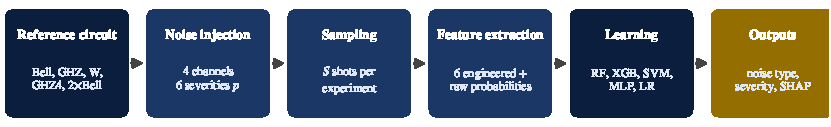
\includegraphics[width=0.85\textwidth]{fig_pipeline.pdf}
\caption{Processing pipeline from reference circuit to noise type, severity and SHAP explanation.}
\label{fig:pipe}
\end{figure*}

\subsection{Datasets}
\emph{Circuits.} Five circuits are used: Bell \cite{nielsen}, GHZ \cite{ghz} and W \cite{dur} states, a 4-qubit GHZ state, and two independent Bell pairs (diagrams in Appendix~A). The last two extend entanglement to four qubits with one connected and two disconnected blocks respectively. Every ideal output has restricted support, so probability found on impossible outcomes is attributable to noise. All qubits are measured in the $Z$ basis.

\emph{Noise channels.} One channel is active per experiment, applied after every gate (1-qubit channel on H, X, $R_y$; 2-qubit channel on CX, CH). \emph{Depolarizing}: random Pauli error with probability $p$. \emph{Amplitude damping}: $|1\rangle\!\to\!|0\rangle$ relaxation with probability $p$ (2-qubit version is the tensor product). \emph{Phase damping}: loss of coherence without population change. \emph{Readout error}: each measured bit is flipped with probability $p$. Severity is $p\in\{0.001,0.005,0.01,0.02,0.03,0.05\}$.

\emph{Generation.} For each circuit, channel, severity and trial ($t=1..6$) the noisy circuit is sampled $S$ times, giving one counts dictionary and one row: $5\times4\times6\times6=720$ rows per dataset (144 per circuit, 180 per class). Seeds are deterministic, so datasets are reproducible. Three independent draws are generated for each of 12 shot settings, giving 36 datasets (720 rows $\times$ 38 columns each: 4 metadata, 6 engineered features, 28 outcome probabilities).

\subsection{Backend and models}
\emph{Backend.} All data come from noisy simulation with Qiskit Aer \cite{qiskit} (\texttt{AerSimulator} with a custom \texttt{NoiseModel}); no quantum hardware was used. \emph{Classifiers.} Random Forest (RF, 300 trees) \cite{breiman}, XGBoost (300 trees, depth 5) \cite{xgb}, SVM with RBF kernel ($C{=}5$), an MLP (64-32 hidden units) and logistic regression (LR); the last three use standardised inputs. Implementations are from scikit-learn \cite{sklearn} and xgboost. A Random Forest regressor estimates the strength $p$ and a 3-class bucket (low $p\le0.005$, medium $\le0.02$, high). Explanations use SHAP \cite{shap}.

\subsection{Features}
Let $P_{\rm o}(s)=\mathrm{count}(s)/S$ be the observed and $P_{\rm id}(s)$ the ideal distribution over $n$-bit strings $s$, with ideal support $\mathcal{S}$. The six engineered features are
\begin{align}
\mathrm{TVD}&=\tfrac12\textstyle\sum_s\big|P_{\rm o}(s)-P_{\rm id}(s)\big|,\\
H&=-\textstyle\sum_s P_{\rm o}(s)\log_2 P_{\rm o}(s),\\
z&=\mathbb{E}_{\rm obs}[f_0]-\mathbb{E}_{\rm id}[f_0],\\
U&=\textstyle\sum_{s\notin\mathcal{S}}P_{\rm o}(s),\\
Q&=\tfrac{1}{U}\textstyle\sum_{\{s,\bar s\}}2\min\{P_{\rm o}(s),P_{\rm o}(\bar s)\},\\
V&=\tfrac12\big(|\Delta P_{\rm even}|+|\Delta P_{\rm odd}|\big),
\end{align}
where $f_0$ is the fraction of 0 bits in a string, $\bar s$ is the bit-complement of $s$ (the sum in $Q$ runs over unordered pairs lying outside $\mathcal{S}$), and $\Delta P_{\rm even/odd}$ is the observed minus ideal probability of even/odd parity. $U$ is the \emph{unexpected-bitstring rate}, $Q$ the \emph{symmetric-swap rate} and $V$ the \emph{parity-violation rate}. The raw features are the per-outcome probabilities (4, 8 and 16 columns for 2-, 3- and 4-qubit outcomes; 28 in total, zero where a circuit lacks that outcome), giving 34 inputs.

\subsection{Metrics}
Primary metric: classification accuracy for the noise type (chance $=25\%$), reported as mean $\pm$ standard deviation over 6 runs (3 independent datasets $\times$ 2 CV seeds) unless stated otherwise. Also reported: per-class and per-severity accuracy, per-circuit accuracy, mean absolute error (MAE) and $R^2$ for the severity regressor, accuracy of the low/medium/high bucket, and joint type-and-bucket accuracy.

\subsection{Train and test settings}
\emph{Default.} 2\,048 shots, 720 rows, default hyperparameters, stratified 5-fold cross-validation. \emph{Pooled} means one model trained on all five circuits; \emph{per-circuit} means a separate model per circuit (144 rows). Each ablation changes one factor at a time from the default (Table~\ref{tab:setup}).

\emph{Row-count ablation.} Subsets are stratified by circuit and noise type and are drawn from the pool of the three 2\,048-shot datasets (2\,160 rows); three subsets per size. At 2\,160 rows the three ``subsets'' coincide, so the reported spread comes from CV seeds only.

\emph{Unseen circuits.} Leave-one-circuit-out (LOCO): train on four circuits, test on the fifth.

\emph{Joint tuning.} A small grid is searched per model (RF 16, XGBoost 12, SVM 12, MLP 6, LR 5 configurations). The best configuration is chosen on datasets 1--2 and evaluated on the independent dataset 3 (3 CV seeds) to avoid selection bias.

\emph{Scope of the protocol.} Random stratified CV puts different shot-noise samples of the \emph{same} circuit--channel--severity configuration in both training and test folds. The reported accuracy therefore measures how well a configuration can be recognised from a fresh sample, not generalisation to unseen severities or circuits; LOCO is the only test of the latter.

\emph{Diagnostic analyses.} To explain the results we use the same datasets without new simulation: (i) confusion matrices of the pooled RF (5-fold CV, 3 datasets); (ii) the number $N=\mathrm{round}(S\cdot U)$ of \emph{off-support shots}, i.e.\ shots whose bitstring is not in the ideal support, and RF accuracy binned by $N$ over all 12 shot settings (phase-damping rows excluded, since they carry almost no off-support events); (iii) mean feature values per channel and the analytic readout-error prediction for Bell; and (iv) a train-on-one-circuit, test-on-another transfer matrix for three feature sets. All are produced by \texttt{analysis.py} in the code repository (Appendix~C).

\begin{table}[!t]
\caption{Experimental settings. Ablated ranges in the last column.}
\label{tab:setup}
\centering\footnotesize\setlength{\tabcolsep}{3pt}
\begin{tabular}{@{}p{1.1in}p{0.5in}p{1.55in}@{}}
\toprule
Factor & Default & Ablated range\\
\midrule
Shots per experiment $S$ & 2\,048 & 50, 100, 200, 400, 600, 720, 1\,024, 2\,048, \dots, 32\,768\\
Rows (experiments) & 720 & 100, 200, \dots, 720, 1\,080, 1\,440, 2\,160\\
Severity $p$ kept & all six & min.\ 0.001 \dots 0.03\\
Circuits in pool & 5 & 1 to 5; leave-one-out\\
Feature set & 34 & raw / engineered / drop-one / single\\
Model hyperparameters & Sec.~V-B & 20 parameters, 5 models\\
CV folds & 5 & 3, 5, 10\\
Independent datasets & 3 & --\\
\bottomrule
\end{tabular}
\end{table}

%==================================================================
\section{Results}\label{sec:results}
\subsection{Noise-type classification}
Table~\ref{tab:main} gives accuracy at the default setting. Random Forest and XGBoost reach 80.2\% and 80.0\% pooled accuracy; SVM, MLP and LR are lower (76.9, 78.3 and 72.0\%). The 4-qubit GHZ circuit is the easiest for every model (88.7--95.3\%), and the single Bell circuit and two Bell pairs the hardest (63.8--74.9\% for RF). Although 4-qubit GHZ and two Bell pairs both use four qubits, one connected entangled block is classified 20 points more accurately than two disconnected pairs: noise on one pair says nothing new about the other.

By class, phase damping is separated almost perfectly (99.3\%), while amplitude damping, depolarizing and readout error are recognised at 73.8, 75.1 and 72.7\%. Phase damping does not change computational-basis populations \cite{nielsen}, so on circuits built from H and CX gates its signature is the \emph{absence} of deviation. This is easy to detect, but it also means the class is recognised as ``no visible deviation''; a noiseless baseline class was not included, so a clean run would likely be confused with it.

\begin{table}[!t]
\caption{Accuracy (\%, mean $\pm$ std over 6 runs) at 2\,048 shots. Pooled: one model for all circuits; circuit columns: separate models. Best per column in bold.}
\label{tab:main}
\centering\scriptsize\setlength{\tabcolsep}{2.2pt}
\begin{tabular}{@{}lccccccc@{}}
\toprule
Model & Pooled & Bell & GHZ & W & GHZ4 & 2$\times$Bell\\
\midrule
RF & \textbf{80.2$\pm$1.1} & 63.8$\pm$3.2 & 85.9$\pm$2.2 & \textbf{86.5$\pm$1.4} & \textbf{95.3$\pm$1.5} & \textbf{74.9$\pm$2.5} \\
XGB & 80.0$\pm$1.2 & 64.8$\pm$2.3 & 84.8$\pm$1.1 & 85.5$\pm$1.9 & 94.1$\pm$1.5 & 70.9$\pm$4.1 \\
SVM & 76.9$\pm$0.6 & \textbf{66.8$\pm$1.9} & 84.1$\pm$2.3 & 84.1$\pm$0.5 & 88.7$\pm$1.4 & 71.6$\pm$1.5 \\
MLP & 78.3$\pm$1.1 & 64.6$\pm$3.3 & 85.6$\pm$2.9 & 85.3$\pm$2.0 & 91.1$\pm$1.5 & 65.2$\pm$4.7 \\
LR & 72.0$\pm$1.1 & 66.8$\pm$1.8 & \textbf{86.0$\pm$1.6} & 86.0$\pm$1.1 & 90.5$\pm$0.8 & 70.0$\pm$2.3 \\
\bottomrule
\end{tabular}
\end{table}

\subsection{Effect of noise strength}
Accuracy rises steeply with $p$ (Fig.~\ref{fig:sevlines}). At 2\,048 shots RF reaches 51.1\% at $p=0.001$, 71.7\% at 0.005, 80.0\% at 0.01 and 95.1\% at 0.03. At $p=0.001$ the average experiment contains only 4.5 off-support shots at 2\,048 shots (0.4 at 200 shots), so weak noise leaves very little signal; Section~\ref{sec:diag} quantifies this.

\begin{figure}[!t]
\centering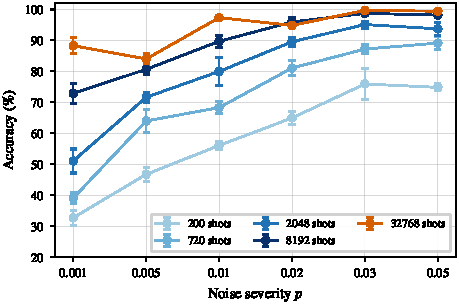
\includegraphics[width=\columnwidth]{fig_sevlines.pdf}
\caption{RF accuracy versus noise severity for five shot counts (mean $\pm$ std over 6 runs).}
\label{fig:sevlines}
\end{figure}

\subsection{Explainability}
Fig.~\ref{fig:shap} shows mean $|$SHAP$|$ values for the Random Forest. The $|0\rangle$ bias $z$ is the most important feature for amplitude damping, matching the one-way $|1\rangle\to|0\rangle$ decay; the symmetric-swap rate $Q$ leads for readout error, whose bit flips produce complementary outcome pairs about equally often (Table~\ref{tab:phys}); depolarizing relies on several features with no clear leader; and phase damping is attributed mainly to the parity-violation and unexpected-bitstring rates, consistent with its near-null signature. The six engineered features carry 56\% of the total attribution although they are only 6 of 34 inputs.

\begin{figure}[!t]
\centering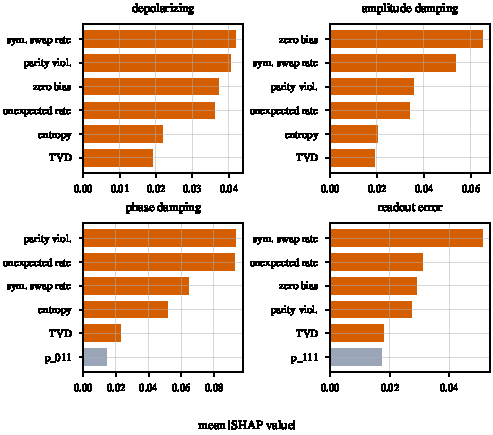
\includegraphics[width=\columnwidth]{fig_shap.pdf}
\caption{Mean $|$SHAP$|$ of the six most important features per class (orange: engineered; grey: raw probabilities).}
\label{fig:shap}
\end{figure}

\subsection{Noise type and strength together}
Over the three datasets, RF predicts the type with $79.8\%$ accuracy, the continuous severity with MAE $=0.0067$ and $R^2=0.59\pm0.02$ (on $\log_{10}p$: $R^2=0.59$), and the low/medium/high bucket with $72.5\%$ accuracy. Both the type and the bucket are correct for $57.3\%$ of experiments. Strength is harder to read than type, again because weak noise is hard to separate from sampling error.

\subsection{Ablation: shots per experiment}
The number of shots is a hyperparameter of the experiment itself. Fig.~\ref{fig:shots} and Table~\ref{tab:shots} sweep $S$ from 50 to 32\,768. Accuracy increases monotonically for all five models: RF goes from 43.9\% (50 shots) to 58.6\% (200), 71.5\% (720), 80.2\% (2\,048), 89.4\% (8\,192) and 94.0\% (32\,768). All models are well above the 25\% chance level even at 50 shots. The 80\% level is crossed at 2\,048 shots by RF and XGBoost, at 4\,096 by SVM and MLP, and at 8\,192 by LR. Accuracy has not saturated at 32\,768 shots; the gain per doubling falls from $+6.2$ points (4\,096$\to$8\,192) to $+2.1$ and $+2.5$ points for the next two doublings. Run-to-run standard deviations are $\le2.8$ points in Table~\ref{tab:shots}, so the ordering is not a sampling artefact. The heat map (Fig.~\ref{fig:heat}) shows where shots help: at $p=0.001$ RF improves from 32.8\% (200 shots) through 51.1\% (2\,048) to 88.3\% (32\,768), whereas at $p\ge0.03$ it is already near 95\% at 2\,048 shots. Phase damping is the most robust class (82.3\% already at 200 shots, 100\% at 32\,768), depolarizing the least (42.0\% at 200 shots).

A least-squares fit of RF accuracy against $\log_2 S$ gives about $+6.9$ points per doubling up to 2\,048 shots and $+3.6$ points per doubling from 2\,048 to 32\,768, so the gain slows down but does not stop. Section~\ref{sec:diag} explains the mechanism.

\begin{figure}[!t]
\centering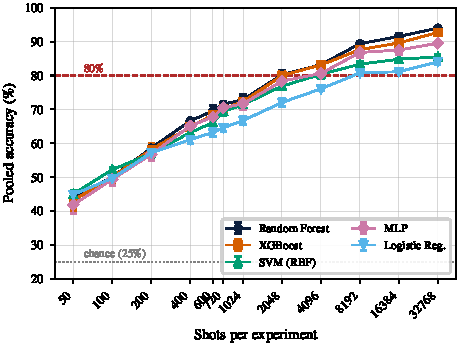
\includegraphics[width=\columnwidth]{fig_shots.pdf}
\caption{Pooled accuracy versus shots per experiment for five models (mean $\pm$ std over 6 runs; 720 rows).}
\label{fig:shots}
\end{figure}

\begin{table}[!t]
\caption{Pooled accuracy (\%) versus shots per experiment (mean $\pm$ std, 6 runs).}
\label{tab:shots}
\centering\scriptsize\setlength{\tabcolsep}{2.5pt}
\begin{tabular}{@{}rccccc@{}}
\toprule
Shots & RF & XGB & SVM & MLP & LR\\
\midrule
50 & 43.9$\pm$1.9 & 43.2$\pm$2.8 & \textbf{45.1$\pm$0.9} & 41.9$\pm$2.5 & 44.9$\pm$1.0 \\
100 & 50.1$\pm$0.7 & 50.0$\pm$1.5 & \textbf{52.2$\pm$0.7} & 49.4$\pm$1.9 & 49.7$\pm$0.7 \\
200 & \textbf{58.6$\pm$1.4} & 58.2$\pm$1.6 & 57.0$\pm$1.0 & 56.8$\pm$1.8 & 57.2$\pm$0.9 \\
400 & \textbf{66.6$\pm$0.7} & 64.8$\pm$1.2 & 63.2$\pm$1.0 & 65.1$\pm$0.9 & 61.1$\pm$1.1 \\
600 & \textbf{69.5$\pm$1.6} & 68.4$\pm$1.0 & 66.1$\pm$1.0 & 67.8$\pm$0.9 & 63.2$\pm$1.1 \\
720 & \textbf{71.5$\pm$0.7} & 70.1$\pm$1.3 & 69.3$\pm$1.0 & 70.5$\pm$0.7 & 64.6$\pm$1.1 \\
1024 & \textbf{72.9$\pm$1.5} & 72.3$\pm$0.7 & 71.4$\pm$0.9 & 71.7$\pm$1.7 & 66.7$\pm$1.2 \\
2048 & \textbf{80.2$\pm$1.1} & 80.0$\pm$1.2 & 76.9$\pm$0.6 & 78.3$\pm$1.1 & 72.0$\pm$1.1 \\
4096 & \textbf{83.2$\pm$0.8} & 83.1$\pm$0.8 & 80.3$\pm$1.2 & 80.6$\pm$0.6 & 76.1$\pm$0.6 \\
8192 & \textbf{89.4$\pm$0.4} & 87.6$\pm$0.9 & 83.3$\pm$0.7 & 86.8$\pm$1.5 & 80.7$\pm$0.8 \\
16384 & \textbf{91.5$\pm$1.0} & 89.6$\pm$0.9 & 84.8$\pm$0.3 & 87.5$\pm$1.3 & 81.1$\pm$0.6 \\
32768 & \textbf{94.0$\pm$0.5} & 92.7$\pm$0.5 & 85.5$\pm$0.6 & 89.5$\pm$0.4 & 84.0$\pm$0.8 \\
\bottomrule
\end{tabular}
\end{table}

\begin{figure*}[!t]
\centering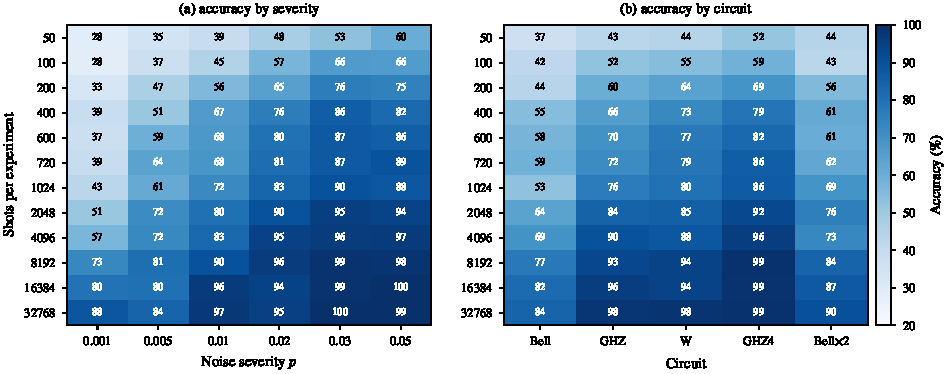
\includegraphics[width=0.9\textwidth]{fig_heat.pdf}
\caption{RF accuracy (\%) as a function of shots per experiment, by (a) noise severity and (b) circuit (pooled model; mean of 6 runs).}
\label{fig:heat}
\end{figure*}

\subsection{Diagnosis: why the accuracy is limited}\label{sec:diag}
\emph{Where the errors are.} Fig.~\ref{fig:conf} shows row-normalised confusion matrices at 2\,048 shots. Phase damping is almost never confused (99\%). For $p\le0.005$ the other three channels are recognised at only 37--57\% and are mostly mistaken for each other, with depolarizing acting as the sink (amplitude damping $\to$ depolarizing 43\%, readout $\to$ depolarizing 44\%); overall accuracy for these rows is 60.3\%. For $p\ge0.02$ the same classifier reaches 92.8\% (81--99\% per class). The overall 80\% is therefore an average of an easy strong-noise regime and a hard weak-noise regime, not a uniform error rate.

\begin{figure}[!t]
\centering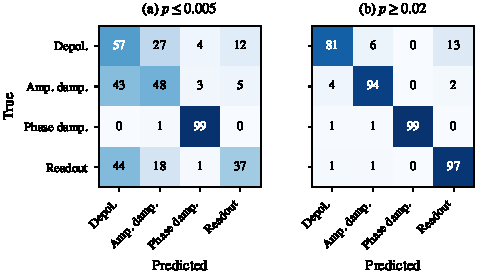
\includegraphics[width=0.95\columnwidth]{fig_conf.pdf}
\caption{Row-normalised confusion matrices (\%) of the pooled RF at 2\,048 shots for (a) weak and (b) strong noise (3 datasets, 5-fold CV).}
\label{fig:conf}
\end{figure}

\emph{Counting the noise signal.} Phase damping aside, every channel moves probability onto outcomes outside the ideal support, so the number $N$ of such shots measures how much evidence an experiment contains. Fig.~\ref{fig:events}(a) shows that $N$ scales linearly with both $S$ and $p$ ($N\approx S\cdot U$). At 200 shots, an experiment at $p=0.001$ contains 0.4 off-support shots on average and 64\% of such experiments contain none; at 2\,048 shots 6\% still contain none, and at 32\,768 shots none do. Fig.~\ref{fig:events}(b) pools all 12 shot settings and shows that accuracy is governed strongly by $N$: 10\% for $N=0$, 37\% for 1--2, 55\% for 6--10, 76\% for 21--50, 90\% for 101--300 and 99.7\% for $N>1000$. When $N=0$ the experiment looks like a noiseless or phase-damping run, and the RF labels 81\% of such rows (at 200 shots) as phase damping. This puts the shot ablation on a mechanistic footing: more shots, or stronger noise, increase $N$. The relation is an association measured across settings; the controlled shot sweep at fixed $p$ (Fig.~\ref{fig:sevlines}) provides the interventional evidence.

\begin{figure*}[!t]
\centering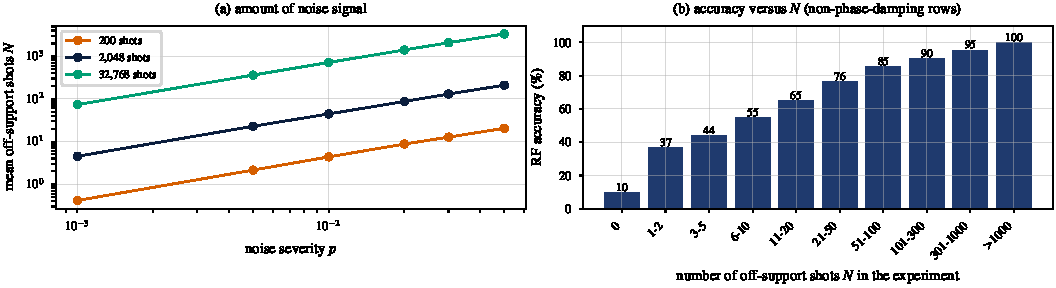
\includegraphics[width=0.9\textwidth]{fig_events.pdf}
\caption{(a) Mean number of off-support shots per experiment (non-phase-damping rows) versus severity. (b) RF accuracy binned by the number $N$ of off-support shots, pooled over all 12 shot settings and 3 datasets (n=1\,163--2\,818 rows per bin).}
\label{fig:events}
\end{figure*}

\emph{Why the three channels are confused.} Table~\ref{tab:phys} lists mean features at $p=0.03$ (32\,768 shots, 5 circuits). The $|0\rangle$ bias $z$ is clearly non-zero only for amplitude damping ($+0.028$, against values within $\pm0.004$ for the other channels), confirming the one-way decay; $Q$ is high for depolarizing and readout (0.86, 0.78) and lower for amplitude damping (0.63), since decay breaks the 0/1 symmetry; phase damping has $U\approx0.001$ and $Q=0$. Magnitude alone does not identify the channel: at equal $p$ the unexpected rate $U$ differs by channel (0.040, 0.058, 0.092), but the values overlap across severities (e.g.\ $U=0.040$ for depolarizing at $p=0.03$ and for amplitude damping at $p=0.02$; Table~\ref{tab:utab} in the Appendix). Channel and strength are thus partly confounded, and the channel must be read from the shape features $z$, $Q$ and $V$, which are estimated from only a handful of events at weak noise. This is the probable reason for the confusions at low $p$; we did not test it with a dedicated experiment. As a check of the simulator, the analytic readout-error rate for the Bell circuit, $U=2p(1-p)$, matches the measured mean at every severity (e.g.\ 0.0199 against 0.0198 at $p=0.01$, 0.0601 against 0.0582 at $p=0.03$, with 18 rows per point).

\begin{table}[!t]
\caption{Mean engineered features per channel at $p=0.03$ (32\,768 shots; 5 circuits, 3 datasets).}
\label{tab:phys}
\centering\scriptsize\setlength{\tabcolsep}{4pt}
\begin{tabular}{@{}lccccc@{}}
\toprule
Channel & TVD & $U$ & $z$ & $Q$ & $V$\\
\midrule
Depolarizing & 0.040 & 0.040 & $-0.003$ & 0.86 & 0.027\\
Amplitude damping & 0.073 & 0.058 & $+0.028$ & 0.63 & 0.052\\
Phase damping & 0.004 & 0.001 & $-0.001$ & 0.00 & 0.000\\
Readout error & 0.092 & 0.092 & $-0.002$ & 0.78 & 0.073\\
\bottomrule
\end{tabular}
\end{table}

\emph{Why transfer to other circuits fails.} Fig.~\ref{fig:transfer} gives the full train-on-one, test-on-another matrix (RF, 2\,048 shots, 144 training rows). With only the six engineered features accuracy is 24--77\%: best between GHZ and GHZ4 (77\%, 69\%), which share the same complementary-pair structure, and worst when testing on the W state (24--46\%), whose ideal support has no complementary pair. With raw probabilities accuracy is at chance (25\%) for every pair except GHZ4$\leftrightarrow$2$\times$Bell (34\%, 45\%), which share two support strings (0000 and 1111). Even GHZ and W, which use identical 3-qubit columns, do not transfer on raw inputs (25.5\%, 26.6\%). This tests and supports the earlier interpretation: the raw columns encode a circuit-specific ideal support, whereas the engineered features are defined relative to the ideal and carry some transferable signal.

\begin{figure}[!t]
\centering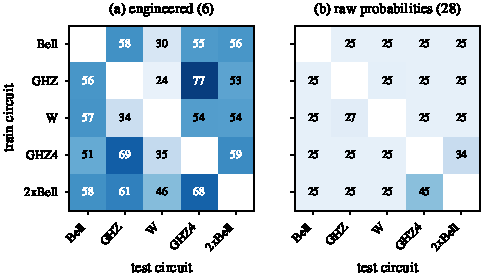
\includegraphics[width=0.95\columnwidth]{fig_transfer.pdf}
\caption{Transfer accuracy (\%) of RF trained on one circuit (row) and tested on another (column) with (a) engineered and (b) raw features. Chance is 25\%.}
\label{fig:transfer}
\end{figure}

\subsection{Ablation: number of rows}
The number of experiments (rows) is varied from 100 to 2\,160 at 2\,048 shots (Fig.~\ref{fig:size}, Table~\ref{tab:size}). RF accuracy grows from 63.7\% (100 rows) to 76.5\% (200), 80.6\% (500), 82.5\% (720) and 84.2\% (2\,160). About 500 rows are needed to pass 80\%; beyond 720 rows the gain is only 1.7 points for a threefold increase. Doubling the shots is far cheaper: 720 rows at 8\,192 shots (four times the simulation cost of the default) give 89.4\%, whereas 2\,160 rows at 2\,048 shots (three times the cost) give 84.2\%. Under a fixed sampling budget, shots are therefore a more efficient resource than additional experiments in this regime. SVM and LR plateau earlier (about 79\% and 74\%). Note that the 720-row subset here (82.5\%) is drawn from the pooled 2\,160 rows and is not the same as the default 720-row dataset (80.2\%); the difference is within one standard deviation of the subset spread.

\begin{figure}[!t]
\centering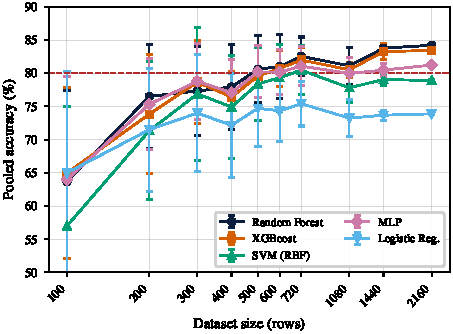
\includegraphics[width=\columnwidth]{fig_size.pdf}
\caption{Pooled accuracy versus number of rows (mean $\pm$ std over 3 subsets).}
\label{fig:size}
\end{figure}

\begin{table}[!t]
\caption{Pooled accuracy (\%) versus number of rows at 2\,048 shots (mean $\pm$ std, 3 subsets).}
\label{tab:size}
\centering\scriptsize\setlength{\tabcolsep}{2.5pt}
\begin{tabular}{@{}rccccc@{}}
\toprule
Rows & RF & XGB & SVM & MLP & LR\\
\midrule
100 & 63.7$\pm$13.7 & \textbf{65.0$\pm$12.8} & 57.0$\pm$18.0 & 64.0$\pm$15.5 & 65.0$\pm$15.3 \\
200 & \textbf{76.5$\pm$7.8} & 73.8$\pm$9.0 & 71.3$\pm$10.4 & 75.3$\pm$6.8 & 71.5$\pm$9.2 \\
300 & 77.3$\pm$6.7 & 78.7$\pm$6.2 & 76.9$\pm$10.0 & \textbf{78.8$\pm$5.7} & 74.0$\pm$8.8 \\
400 & \textbf{77.9$\pm$6.4} & 76.4$\pm$3.9 & 74.9$\pm$7.8 & 77.1$\pm$5.0 & 72.2$\pm$7.9 \\
500 & \textbf{80.6$\pm$5.1} & 79.6$\pm$4.5 & 78.4$\pm$5.5 & 80.2$\pm$3.9 & 74.7$\pm$5.8 \\
600 & \textbf{81.0$\pm$4.8} & 80.7$\pm$2.7 & 79.3$\pm$5.0 & 80.2$\pm$3.4 & 74.3$\pm$4.6 \\
720 & \textbf{82.5$\pm$2.9} & 82.0$\pm$1.9 & 80.5$\pm$3.7 & 81.1$\pm$3.0 & 75.4$\pm$3.4 \\
1080 & \textbf{81.1$\pm$2.8} & 80.5$\pm$1.1 & 77.8$\pm$2.3 & 80.0$\pm$2.4 & 73.2$\pm$2.8 \\
1440 & \textbf{83.8$\pm$0.5} & 83.3$\pm$1.1 & 79.1$\pm$0.8 & 80.5$\pm$0.9 & 73.7$\pm$0.7 \\
2160 & \textbf{84.2$\pm$0.3} & 83.4$\pm$0.1 & 78.9$\pm$0.1 & 81.2$\pm$0.4 & 73.9$\pm$0.2 \\
\bottomrule
\end{tabular}
\end{table}

\subsection{Ablation: severity range and circuit family}
Keeping only rows with $p\ge p_{\min}$ (Fig.~\ref{fig:sevcirc}a) raises RF accuracy from 80.2\% ($p_{\min}=0.001$) to 86.0, 90.4, 95.8 and 98.9\% ($p_{\min}=0.03$): the weakest noise causes most errors. Growing the pool of circuits (Fig.~\ref{fig:sevcirc}b: Bell; $+$GHZ; $+$W; $+$GHZ4; $+$two Bell pairs) improves pooled accuracy from 63.8\% to 82.6\% with four circuits, then lowers it to 80.2\% when two Bell pairs are added.

We also test transfer to an \emph{unseen} circuit (Table~\ref{tab:loco}). Transfer is weak with all 34 features (22.9--69.2\%; below chance for W) and better with the six engineered features alone (40.0--75.0\%). The pairwise transfer matrix (Fig.~\ref{fig:transfer}) shows why: raw probabilities are tied to each circuit's ideal support and transfer at chance level unless the supports overlap. A model should therefore be trained on the circuit family it will be applied to.

\begin{figure}[!t]
\centering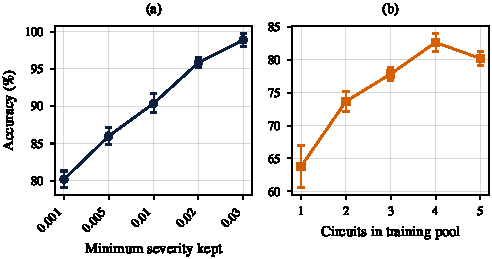
\includegraphics[width=\columnwidth]{fig_sevcirc.pdf}
\caption{(a) RF accuracy when only severities $\ge p_{\min}$ are kept. (b) Accuracy versus number of circuits in the training pool. Mean $\pm$ std over 6 runs.}
\label{fig:sevcirc}
\end{figure}

\begin{table}[!t]
\caption{Leave-one-circuit-out accuracy (\%) of RF (mean $\pm$ std, 3 datasets).}
\label{tab:loco}
\centering\footnotesize
\begin{tabular}{@{}lcc@{}}
\toprule
Held-out circuit & All 34 features & Engineered only\\
\midrule
Bell & 58.6$\pm$1.2 & 63.0$\pm$1.8 \\
GHZ & 53.2$\pm$2.8 & 63.0$\pm$0.9 \\
W state & 22.9$\pm$5.6 & 40.0$\pm$4.3 \\
GHZ4 & 69.2$\pm$1.7 & 75.0$\pm$0.6 \\
2$\times$Bell & 59.3$\pm$1.8 & 70.6$\pm$1.2 \\
\bottomrule
\end{tabular}
\end{table}

\subsection{Ablation: feature set}
Fig.~\ref{fig:feat} compares feature sets for RF. Raw probabilities alone give 79.3\% and engineered features alone 75.8\%, against 80.2\% for both. Removing any single engineered feature changes accuracy by at most 0.6 points, within one standard deviation, so the six features are largely redundant with one another and with the raw probabilities. Individually, the symmetric-swap rate is the most informative (56.3\%) and the $|0\rangle$ bias the least (35.3\%) for the pooled four-class task; $z$ matters mainly for the amplitude-damping class (Fig.~\ref{fig:shap}). The engineered features add 0.9 points over raw probabilities but make the model interpretable.

\begin{figure}[!t]
\centering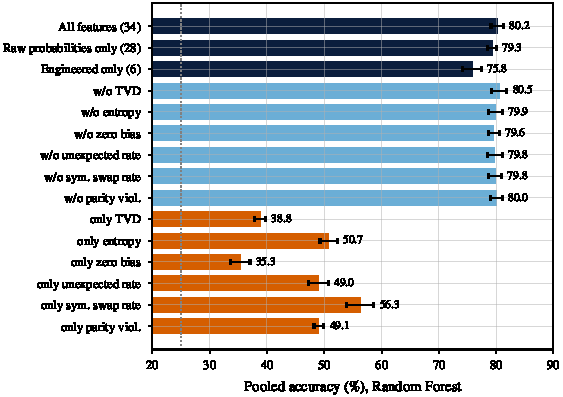
\includegraphics[width=\columnwidth]{fig_feat.pdf}
\caption{RF accuracy for different feature sets (mean $\pm$ std over 6 runs; dotted line: chance).}
\label{fig:feat}
\end{figure}

\subsection{Ablation: classifier hyperparameters}
Each hyperparameter is varied alone from the default, evaluated on all three datasets (Fig.~\ref{fig:hp1}, \ref{fig:hp2}); Fig.~\ref{fig:sens} ranks them by the range of accuracy they produce.

\emph{Random Forest.} The number of trees is irrelevant from 10 to 500 (79.4--80.2\%). Depth is the only strong parameter: 66.3, 74.2, 78.6\% for depth 2, 4, 6, and $\ge79.9\%$ from depth 8. Considering all features at each split instead of $\sqrt{n}$ costs 2.1 points; criterion, bootstrap and minimum split size change accuracy by $\le0.9$ points. \emph{XGBoost.} All values fall within 77.8--80.0\%; only the smallest learning rate (0.01, undertrained at 300 trees) is lower. \emph{SVM.} The most sensitive model: kernel (RBF 77.1\%, sigmoid 56.1\%), $C$ (57.9\% at 0.1 to 78.0\% at 50) and $\gamma$ (64.7\% at $10^{-3}$, 77.7\% at 0.1, 71.1\% at 1) change accuracy by 13--21 points. \emph{MLP.} Width and depth are irrelevant (78.6--79.1\%); only the logistic activation (75.5\%) and the smallest learning rate (77.8\%) lose accuracy. \emph{LR.} Strong regularisation hurts: 60.0\% at $C=10^{-3}$ rising to 72.9\% at $C=100$.

\begin{figure}[!tb]
\centering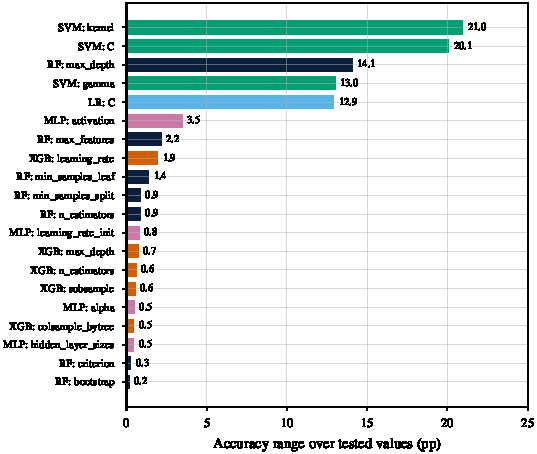
\includegraphics[width=\columnwidth]{fig_sens.pdf}
\caption{Accuracy range (max $-$ min of the mean) produced by each hyperparameter.}
\label{fig:sens}
\end{figure}

\begin{figure*}[!t]
\centering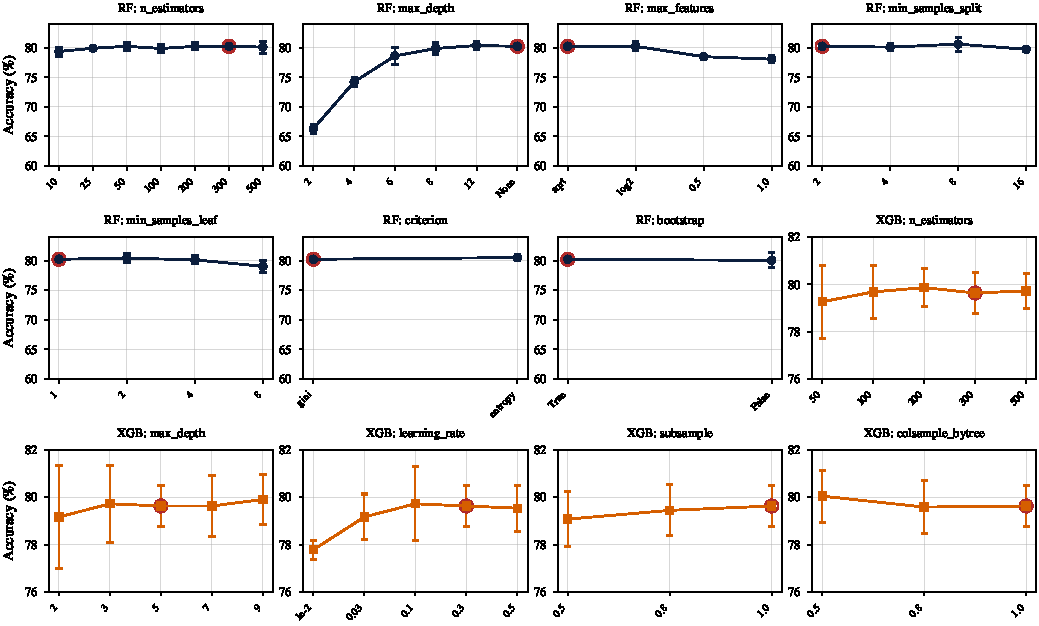
\includegraphics[width=\textwidth]{fig_hp_trees.pdf}
\caption{Single-hyperparameter ablation for RF (top two rows) and XGBoost (bottom row); mean $\pm$ std over 3 datasets, red circle: default value.}
\label{fig:hp1}
\end{figure*}

\begin{figure*}[!t]
\centering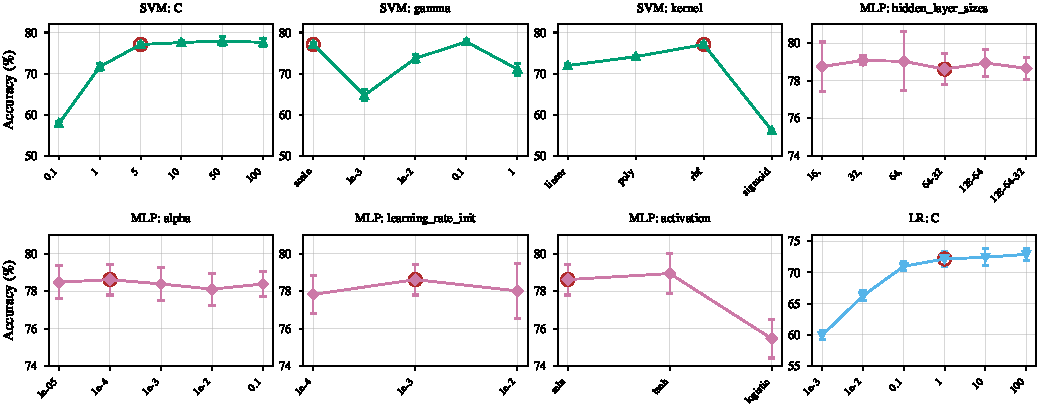
\includegraphics[width=\textwidth]{fig_hp_other.pdf}
\caption{Single-hyperparameter ablation for SVM, MLP and LR; mean $\pm$ std over 3 datasets, red circle: default value.}
\label{fig:hp2}
\end{figure*}

\subsection{Joint tuning and cross-validation folds}
Table~\ref{tab:tune} shows that tuning does not reliably help tree ensembles: the selected RF and XGBoost settings lose 0.8 and 1.3 points on the held-out dataset, comparable to one standard deviation, i.e.\ selection noise. For SVM and LR the apparent gains ($+0.9$ and $+1.8$) depend on how exact ties in the selection score were broken: $C=5$ and $C=10$ (SVM, $\gamma=0.1$) and $C=10$ and $C=100$ (LR) have identical mean accuracy on datasets 1--2. Choosing the other tied value gives $+0.3$ and $+0.0$ (Table~\ref{tab:tune}). We therefore regard the gain for SVM and LR as small and uncertain. For the MLP the default itself is selected. Varying the number of CV folds changes RF accuracy only from 79.3\% (3 folds) to 80.2\% (5) and 80.7\% (10), and does not change the model ranking.

\begin{table}[!t]
\caption{Joint tuning: configuration chosen on datasets 1--2 and accuracy (\%) on held-out dataset 3 (mean $\pm$ std, 3 CV seeds). $^\dagger$Exact tie on datasets 1--2; the alternative tied value is shown in the last column.}
\label{tab:tune}
\centering\scriptsize\setlength{\tabcolsep}{2pt}
\begin{tabular}{@{}llccc@{}}
\toprule
Model & Selected configuration & Default & Selected & Tied alt.\\
\midrule
RF & n=100, d=None, mf=sqrt, msl=2 & 80.8$\pm$0.9 & 80.0$\pm$1.0 & --\\
XGB & d=7, lr=0.1, n=100 & 80.1$\pm$1.0 & 78.8$\pm$1.0 & --\\
SVM$^\dagger$ & C=10, $\gamma$=0.1 & 77.1$\pm$0.2 & 78.0$\pm$0.7 & 77.4$\pm$0.5 (C=5)\\
MLP & hid=(64,32), $\alpha$=1e-4 & 78.1$\pm$0.5 & 78.1$\pm$0.5 & --\\
LR$^\dagger$ & C=100 & 70.8$\pm$0.2 & 72.6$\pm$0.1 & 70.8$\pm$0.2 (C=10)\\
\bottomrule
\end{tabular}
\end{table}

\subsection{Summary of effects}
Table~\ref{tab:effects} orders the factors by the accuracy range they produce for RF. Shots, the number of rows, the severity range and the circuit pool dominate; among model choices, the classifier family and the forest depth matter most. SVM kernel and $C$ matter more than any tree hyperparameter (13--21 points), but SVM stays below RF in its best setting.

\emph{Why hyperparameters matter little.} Five very different learners end within 8 points of each other at 2\,048 shots, RF and XGBoost within 0.2 points, whereas the shot count moves the same RF by 50 points. This pattern indicates that accuracy is limited by the information in the counts (Fig.~\ref{fig:events}) rather than by model capacity; this is an inference from the ablations, not a separate test. The sensitivity of the SVM is the usual behaviour of an RBF kernel on 34 standardised inputs, where $\gamma$ and $C$ set the smoothness of the boundary; we did not study it further.

\begin{table}[!t]
\caption{Effect of each factor on RF accuracy (percentage points).}
\label{tab:effects}
\centering\scriptsize\setlength{\tabcolsep}{3pt}
\begin{tabular}{@{}lccc@{}}
\toprule
Factor & Range tested & Accuracy range (\%) & Effect\\
\midrule
Shots per experiment & 50--32\,768 & 43.9--94.0 & 50.1\\
Rows & 100--2\,160 & 63.7--84.2 & 20.5\\
Minimum severity kept & 0.001--0.03 & 80.2--98.9 & 18.7\\
Circuits in pool & 1--5 & 63.8--82.6 & 18.8\\
RF max depth & 2--None & 66.3--80.4 & 14.1\\
Classifier family (2\,048 shots) & 5 models & 72.0--80.2 & 8.2\\
Feature set (multi-feature) & 3 sets & 75.8--80.2 & 4.4\\
Other RF hyperparameters & -- & 78.1--80.6 & $\le$2.5\\
CV folds & 3, 5, 10 & 79.3--80.7 & 1.4\\
\bottomrule
\end{tabular}
\end{table}

\subsection{Implications for error mitigation}\label{sec:mitig}
A classifier that names the dominant channel and its rough strength suggests which mitigation to try (Table~\ref{tab:mitig}). Readout error is corrected after measurement with a calibration matrix \cite{bravyi}; dephasing is suppressed by dynamical decoupling \cite{viola}; depolarizing and coherent errors are converted to stochastic noise by randomized compiling \cite{wallman}; amplitude damping grows with circuit duration, so shorter circuits and $T_1$-aware scheduling are the lever. Because the strength estimate is least reliable for $p\le0.005$, this guidance is least dependable exactly where noise is already small. These recommendations are standard practice and were not tested experimentally here.

\begin{table}[!t]
\caption{Predicted channel and suggested mitigation.}
\label{tab:mitig}
\centering\footnotesize
\begin{tabular}{@{}ll@{}}
\toprule
Channel & Mitigation\\
\midrule
Depolarizing & randomized compiling / Pauli twirling \cite{wallman}\\
Amplitude damping & shorter circuits, $T_1$-aware scheduling\\
Phase damping & dynamical decoupling \cite{viola}\\
Readout error & calibration-matrix correction \cite{bravyi}\\
\bottomrule
\end{tabular}
\end{table}

%==================================================================
\section{Conclusion and Outlook}\label{sec:concl}
Computational-basis counts of small entangled circuits carry enough information to recognise the dominant noise channel in simulation: Random Forest reaches $80.2\pm1.1\%$ pooled accuracy at 2\,048 shots, up to $95.3\%$ with per-circuit models (4-qubit GHZ), and $98.9\%$ when only $p\ge0.03$ is considered. The ablation shows that accuracy is governed chiefly by data: shots (+50 points over the tested range), the number of rows (+20 points) and the circuit pool, while hyperparameters play a minor role (tree ensembles within about 2 points once depth is at least 8, the MLP within 3.5 points; SVM and LR need a suitable kernel and regularisation). Tuning did not improve held-out accuracy for tree ensembles, and its small gains for SVM and LR are tie-dependent. SHAP shows that the engineered features act as intended. The diagnostics explain the limits: errors concentrate in weak-noise confusions among depolarizing, amplitude-damping and readout noise, and accuracy tracks the number of off-support shots (10\% with none, 99.7\% with more than 1\,000), so the ceiling is set by the information in the counts rather than by the classifier.

\emph{Scope and limitations.} Results come from noise simulation with one channel at a time, five circuits, $Z$-basis measurement and random stratified CV, which shares configurations between training and test folds. Cross-circuit transfer is limited (Table~\ref{tab:loco}), phase damping is detected as the absence of deviation, and no noiseless class or real-hardware data are included.

\emph{Outlook.} Next steps are validation on IBM hardware against published calibration data, a noiseless baseline class and combined (multi-channel) noise, an $X$-basis variant to make phase damping visible, larger circuits, evaluation on held-out severities, and a comparison with quantum-kernel classifiers to test whether a quantum learner adds anything for this task.

%==================================================================
\begin{thebibliography}{99}
\bibitem{preskill} J. Preskill, ``Quantum computing in the NISQ era and beyond,'' \emph{Quantum}, vol. 2, p. 79, 2018.
\bibitem{bharti} K. Bharti \emph{et al.}, ``Noisy intermediate-scale quantum algorithms,'' \emph{Rev. Mod. Phys.}, vol. 94, no. 1, art. 015004, 2022.
\bibitem{chuang} I. L. Chuang and M. A. Nielsen, ``Prescription for experimental determination of the dynamics of a quantum black box,'' \emph{J. Mod. Opt.}, vol. 44, no. 11--12, pp. 2455--2467, 1997.
\bibitem{blume} R. Blume-Kohout \emph{et al.}, ``Demonstration of qubit operations below a rigorous fault tolerance threshold with gate set tomography,'' \emph{Nat. Commun.}, vol. 8, art. 14485, 2017.
\bibitem{martina} S. Martina, L. Buffoni, S. Gherardini, and F. Caruso, ``Learning the noise fingerprint of quantum devices,'' \emph{Quantum Mach. Intell.}, vol. 4, art. 8, 2022.
\bibitem{jain} V. Jain and L. Zhang, ``Shadow-based noise fingerprinting of simulated quantum noise models,'' arXiv:2607.08998, 2026.
\bibitem{magesan} E. Magesan, J. M. Gambetta, and J. Emerson, ``Scalable and robust randomized benchmarking of quantum processes,'' \emph{Phys. Rev. Lett.}, vol. 106, no. 18, art. 180504, 2011.
\bibitem{harper} R. Harper, S. T. Flammia, and J. J. Wallman, ``Efficient learning of quantum noise,'' \emph{Nat. Phys.}, vol. 16, pp. 1184--1188, 2020.
\bibitem{huang} H.-Y. Huang, R. Kueng, and J. Preskill, ``Predicting many properties of a quantum system from very few measurements,'' \emph{Nat. Phys.}, vol. 16, no. 10, pp. 1050--1057, 2020.
\bibitem{simshadow} A. Bensoussan, E. Chachkarova, K. Even-Mendoza, S. Fortz, V. Klimis, and M. R. Mousavi, ``Toward live noise fingerprinting in quantum software engineering,'' arXiv:2512.18667, 2025.
\bibitem{zlokapa} A. Zlokapa and A. Gheorghiu, ``A deep learning model for noise prediction on near-term quantum devices,'' arXiv:2005.10811, 2020.
\bibitem{strikis} A. Strikis, D. Qin, Y. Chen, S. C. Benjamin, and Y. Li, ``Learning-based quantum error mitigation,'' arXiv:2005.07601, 2020.
\bibitem{bravyi} S. Bravyi, S. Sheldon, A. Kandala, D. C. McKay, and J. M. Gambetta, ``Mitigating measurement errors in multiqubit experiments,'' \emph{Phys. Rev. A}, vol. 103, art. 042605, 2021.
\bibitem{temme} K. Temme, S. Bravyi, and J. M. Gambetta, ``Error mitigation for short-depth quantum circuits,'' \emph{Phys. Rev. Lett.}, vol. 119, art. 180509, 2017.
\bibitem{viola} L. Viola, E. Knill, and S. Lloyd, ``Dynamical decoupling of open quantum systems,'' \emph{Phys. Rev. Lett.}, vol. 82, no. 12, pp. 2417--2421, 1999.
\bibitem{wallman} J. J. Wallman and J. Emerson, ``Noise tailoring for scalable quantum computation via randomized compiling,'' \emph{Phys. Rev. A}, vol. 94, art. 052325, 2016.
\bibitem{nielsen} M. A. Nielsen and I. L. Chuang, \emph{Quantum Computation and Quantum Information}, 10th anniv. ed. Cambridge, U.K.: Cambridge Univ. Press, 2010.
\bibitem{ghz} D. M. Greenberger, M. A. Horne, and A. Zeilinger, ``Going beyond Bell's theorem,'' in \emph{Bell's Theorem, Quantum Theory and Conceptions of the Universe}, M. Kafatos, Ed. Dordrecht, The Netherlands: Kluwer, 1989, pp. 69--72.
\bibitem{dur} W. D\"ur, G. Vidal, and J. I. Cirac, ``Three qubits can be entangled in two inequivalent ways,'' \emph{Phys. Rev. A}, vol. 62, no. 6, art. 062314, 2000.
\bibitem{qiskit} H. Abraham \emph{et al.}, ``Qiskit: An open-source framework for quantum computing,'' Zenodo, 2019, doi:10.5281/zenodo.2573505.
\bibitem{breiman} L. Breiman, ``Random forests,'' \emph{Mach. Learn.}, vol. 45, no. 1, pp. 5--32, 2001.
\bibitem{xgb} T. Chen and C. Guestrin, ``XGBoost: A scalable tree boosting system,'' in \emph{Proc. ACM SIGKDD}, 2016, pp. 785--794.
\bibitem{sklearn} F. Pedregosa \emph{et al.}, ``Scikit-learn: Machine learning in Python,'' \emph{J. Mach. Learn. Res.}, vol. 12, pp. 2825--2830, 2011.
\bibitem{shap} S. M. Lundberg and S.-I. Lee, ``A unified approach to interpreting model predictions,'' in \emph{Proc. NeurIPS}, 2017, pp. 4765--4774.
\end{thebibliography}

%==================================================================
\appendices
\section{Circuit Diagrams}\label{app:circ}
Fig.~\ref{fig:circuits} shows the five reference circuits and their ideal output distributions. All qubits are measured in the $Z$ basis after the gates shown; the gate set is H, X, $R_y$, CX and CH. The W state uses $R_y(1.9106)$, a controlled-Hadamard, two CX gates and an X gate.

\begin{figure}[!h]
\centering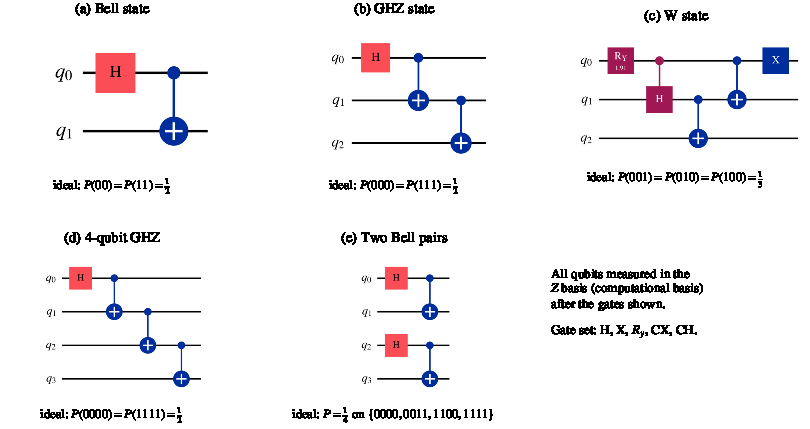
\includegraphics[width=\columnwidth]{fig_circuits.pdf}
\caption{The five reference circuits and their ideal output distributions: (a) Bell, (b) GHZ, (c) W, (d) 4-qubit GHZ, (e) two Bell pairs.}
\label{fig:circuits}
\end{figure}

\section{Supporting Tables}\label{app:tables}
\begin{table}[!h]
\caption{RF per-class accuracy (\%, pooled, mean of 6 runs) versus shots.}
\label{tab:class}
\centering\scriptsize\setlength{\tabcolsep}{3pt}
\begin{tabular}{@{}rcccc@{}}
\toprule
Shots & Amp.\ damp. & Depolarizing & Phase damp. & Readout\\
\midrule
200 & 51.4 & 42.0 & 82.3 & 58.6\\
2\,048 & 73.8 & 75.1 & 99.3 & 72.7\\
32\,768 & 93.7 & 92.0 & 100.0 & 90.1\\
\bottomrule
\end{tabular}
\end{table}

\begin{table}[!h]
\caption{Top-3 features by mean $|$SHAP$|$ per class (RF, 2\,048 shots).}
\label{tab:shaptab}
\centering\scriptsize\setlength{\tabcolsep}{3pt}
\begin{tabular}{@{}ll@{}}
\toprule
Class & Top features (mean $|$SHAP$|$)\\
\midrule
Depolarizing & $Q$ (0.042), $V$ (0.041), $z$ (0.037)\\
Amplitude damping & $z$ (0.065), $Q$ (0.053), $V$ (0.036)\\
Phase damping & $V$ (0.093), $U$ (0.093), $Q$ (0.065)\\
Readout error & $Q$ (0.051), $U$ (0.031), $z$ (0.029)\\
\bottomrule
\end{tabular}
\end{table}

\begin{table}[!h]
\caption{Mean unexpected-bitstring rate $U$ by channel and severity (32\,768 shots; 5 circuits, 3 datasets).}
\label{tab:utab}
\centering\scriptsize\setlength{\tabcolsep}{3pt}
\begin{tabular}{@{}lcccccc@{}}
\toprule
$p$ & 0.001 & 0.005 & 0.01 & 0.02 & 0.03 & 0.05\\
\midrule
Depolarizing & 0.0014 & 0.0068 & 0.0135 & 0.0271 & 0.0401 & 0.0660\\
Amp.\ damping & 0.0021 & 0.0104 & 0.0204 & 0.0396 & 0.0578 & 0.0914\\
Phase damping & 0.0000 & 0.0002 & 0.0003 & 0.0007 & 0.0010 & 0.0017\\
Readout error & 0.0032 & 0.0159 & 0.0315 & 0.0620 & 0.0917 & 0.1482\\
\bottomrule
\end{tabular}
\end{table}

\begin{table}[!h]
\caption{Single-hyperparameter grids (default in Sec.~V-B; one parameter varied at a time).}
\label{tab:hpgrid}
\centering\scriptsize\setlength{\tabcolsep}{2pt}
\begin{tabular}{@{}lp{2.5in}@{}}
\toprule
Model & Values tried\\
\midrule
RF & trees 10--500; depth 2, 4, 6, 8, 12, None; max\_features sqrt, log2, 0.5, 1.0; min split 2--16; min leaf 1--8; criterion gini/entropy; bootstrap T/F\\
XGB & trees 50--500; depth 2--9; lr 0.01--0.5; subsample 0.5--1; colsample 0.5--1\\
SVM & $C$ 0.1--100; $\gamma$ scale, $10^{-3}$--1; kernel linear/poly/rbf/sigmoid\\
MLP & hidden (16,) to (128,64,32); $\alpha$ $10^{-5}$--0.1; lr $10^{-4}$--0.01; relu/tanh/logistic\\
LR & $C$ $10^{-3}$--100\\
\bottomrule
\end{tabular}
\end{table}

\section{Code Availability and Reproducibility}\label{app:code}
All source code, the 36 seeded datasets (\texttt{datasets/s<shots>\_d<draw>.csv}), the raw per-evaluation results of every ablation (\texttt{results/*.jsonl}) and the figure scripts are available at

\begin{center}\small\url{https://github.com/Nitheka07/ML-Based-Noise-Source-Fingerprinting-for-Quantum-Circuits}\end{center}

The repository is organised as \texttt{code/} (circuits, noise models, features, models, ablations, diagnostics, figures), \texttt{datasets/}, \texttt{results/}, \texttt{figs/} and \texttt{paper/}. Usage, run from the repository root: \texttt{python code/gen\_all.py 600} regenerates the datasets; \texttt{python code/runexp.py <exp> 600} runs an ablation (\texttt{exp} $\in$ \{shots, size, feat, sev, circ, hp, cv, main, tune\}); \texttt{python code/analysis.py} runs the diagnostics; \texttt{python code/figs.py} redraws the figures. All paths are resolved relative to the repository folder. Required: Python 3.9+, qiskit, qiskit-aer, scikit-learn, xgboost, shap, pandas, numpy, matplotlib. Library versions (Qiskit, Aer, scikit-learn, xgboost) were not recorded when the results were produced, so small numerical differences are possible with other versions.

\end{document}
